\chapter{REFERENCIAL TEÓRICO}\label{sec:referencial}

Esta seção apresenta o modelo de bicicleta, o ângulo de deriva e os métodos para estimá-lo, e os fundamentos de aprendizado supervisionado, programação genética e MGGP em que o trabalho se apoia.

\section{Modelagem veicular e modelo de bicicleta}\label{sec:modelagem_veiculos}

No âmbito deste trabalho, adota-se o modelo de bicicleta, que simplifica o veículo considerando apenas dois pontos de contato com o solo: um no eixo dianteiro e outro no eixo traseiro. O Centro de Gravidade (CG), situado entre esses dois eixos, é tomado como o ponto de referência para a modelagem cinemática. Esse modelo é utilizado devido à sua formulação matemática e capacidade de capturar o comportamento dinâmico do veículo no plano horizontal \cite{viehweger2020}.

A modelagem considera que o veículo pode se mover longitudinalmente ($v_x$) e lateralmente ($v_y$) em relação ao CG, ao mesmo tempo em que realiza rotações em torno de seu eixo vertical, uma grandeza caracterizada pela taxa de guinada ($\dot{\psi}$). Em momentos em que ocorre o esterçamento das rodas dianteiras (ângulo $\delta$) a fim de deslocar o veículo lateralmente, surgem os ângulos de deslizamento da roda dianteira ($\alpha_f$) e da roda traseira ($\alpha_r$), bem como o ângulo de deslizamento lateral do veículo, também denominado ângulo de deriva ($\beta$) \cite{rajamani2012}.

A velocidade longitudinal está associada ao deslocamento na direção do eixo longitudinal do veículo. A variação da velocidade longitudinal ($\dot{v}_x$), expressa pela \autoref{eq:velocidade_longitudinal}, depende da aceleração medida nessa direção e do efeito rotacional combinado à velocidade lateral \cite{jiang2019}:
\begin{equation}
    \dot{v}_x = a_x + \dot{\psi} v_y.
    \label{eq:velocidade_longitudinal}
\end{equation}

A velocidade lateral representa o desvio perpendicular ao eixo longitudinal, sendo resultante de manobras de esterçamento ou forças de perturbação lateral. A variação da velocidade lateral ($\dot{v}_y$), detalhada na \autoref{eq:velocidade_lateral}, relaciona a aceleração lateral à interação existente entre a rotação do veículo e sua velocidade longitudinal \cite{jiang2019}:
\begin{equation}
    \dot{v}_y = a_y - \dot{\psi} v_x.
    \label{eq:velocidade_lateral}
\end{equation}

Na \autoref{fig:modelo_bicicleta}, apresenta-se a representação do modelo de bicicleta, cuja estrutura serviu de base geométrica e cinemática para a modelagem proposta neste trabalho.

\begin{figure}[htbp]
    \centering
    \caption{Modelo de bicicleta para a cinemática veicular, com o ângulo de deriva $\beta$ entre o vetor velocidade $V$ no CG e o eixo longitudinal.}
    \label{fig:modelo_bicicleta}
    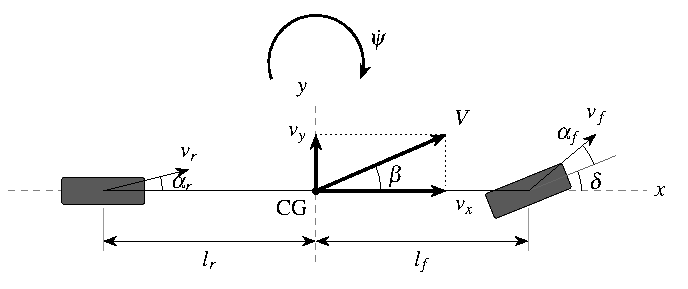
\includegraphics[width=0.85\textwidth]{figuras/diagramas/modelo_bicicleta.pdf}
    \fonte{Elaboração própria, adaptado de \citeonline{rajamani2012}.}
\end{figure}

\section{Ângulo de deriva}\label{sec:angulo_deriva}

O ângulo de deriva é o ângulo entre o vetor velocidade do veículo no CG e o seu eixo longitudinal (\autoref{fig:modelo_bicicleta}). Em função das componentes da velocidade, ele é definido por
\begin{equation}
    \beta = \operatorname{atan2}(v_y, v_x) \approx \frac{v_y}{v_x},
    \label{eq:beta}
\end{equation}
em que a aproximação vale para ângulos pequenos e $v_x > 0$, condição típica da condução normal, na qual $\beta$ raramente ultrapassa alguns graus \cite{rajamani2012}.

Derivando a aproximação da \autoref{eq:beta} no tempo e substituindo as Equações \ref{eq:velocidade_longitudinal} e \ref{eq:velocidade_lateral}, desprezando-se os termos de segunda ordem em $\beta$ e a variação de $v_x$, obtém-se a relação cinemática
\begin{equation}
    \dot{\beta} \approx \frac{a_y}{v_x} - \dot{\psi},
    \label{eq:beta_cinematica}
\end{equation}
que relaciona a evolução do ângulo de deriva a duas grandezas medidas por uma unidade inercial ($a_y$ e $\dot\psi$) e à velocidade longitudinal. A \autoref{eq:beta_cinematica} não depende de parâmetros do pneu nem do veículo, mas exige integração: qualquer viés em $a_y$ ou $\dot\psi$ se acumula ao longo do tempo, e o termo $a_y/v_x$ torna-se mal condicionado em baixa velocidade. Pelo mesmo motivo, o cálculo de $\beta$ por $\operatorname{atan2}(\hat v_y, \hat v_x)$ amplifica o erro de $\hat v_y$ quando $v_x$ é pequeno: um erro $\varepsilon$ em $v_y$ produz um erro aproximado de $\varepsilon / v_x$ em $\beta$.

O ângulo de deriva é uma das variáveis centrais do controle de estabilidade veicular. Valores elevados de $\beta$ indicam que o veículo está próximo do limite de aderência dos pneus e que sua resposta ao volante deixa de ser previsível; por isso, sistemas de controle de estabilidade procuram manter $\beta$ dentro de limites seguros. Como sensores capazes de medir $\beta$ diretamente --- sensores ópticos de velocidade ou sistemas GPS/INS de alta precisão --- têm custo elevado para veículos de série, $\beta$ é, em geral, estimado a partir dos sensores convencionais do veículo \cite{chindamo2018}.

\section{Métodos de estimação do ângulo de deriva}\label{sec:metodos_estimacao}

A literatura organiza os estimadores de ângulo de deriva em três famílias principais \cite{chindamo2018, liu2018}.

Os métodos baseados em modelo cinemático usam apenas relações geométricas e cinemáticas, como a \autoref{eq:beta_cinematica}, alimentadas por acelerômetros, giroscópios e velocidades das rodas. Sua vantagem é a independência de parâmetros do veículo e do pneu; sua desvantagem é a sensibilidade a vieses e ruídos dos sensores, que, integrados, fazem a estimativa derivar ao longo do tempo. Por isso, costumam ser combinados com alguma forma de correção, como medidas de GPS \cite{liu2018}.

Os métodos baseados em modelo dinâmico descrevem as forças laterais nos pneus e usam observadores --- filtros de Kalman e suas variantes, observadores de modos deslizantes, observadores não lineares --- para estimar $\beta$. São precisos dentro da faixa de validade do modelo, mas dependem de parâmetros como a rigidez lateral dos pneus e o coeficiente de atrito com o pavimento, que variam com a carga, o desgaste e a condição da pista \cite{puscul2024}.

Os métodos orientados a dados aprendem a relação entre as medições disponíveis e $\beta$ a partir de ensaios de referência, frequentemente com redes neurais. Dispensam modelos explícitos, mas, em geral, produzem modelos do tipo caixa-preta, de difícil interpretação e certificação \cite{chindamo2018}. A Programação Genética Multigene ocupa uma posição intermediária: é orientada a dados, mas produz equações simbólicas que podem ser inspecionadas e comparadas com a física do problema, como fez a IC para as velocidades. Este trabalho investiga se essa abordagem pode fornecer o ângulo de deriva diretamente, como saída do modelo.

\section{Aprendizado supervisionado e programação genética}

O aprendizado de máquina (\textit{Machine Learning}), uma das subáreas da IA, capacita sistemas computacionais a alterar seu desempenho a partir de dados \cite{filho2024}. No aprendizado supervisionado, paradigma adotado neste trabalho, o modelo é treinado com dados rotulados, em que cada entrada está associada a uma saída conhecida, e deve generalizar essa relação para dados inéditos \cite{pecht2021}. Essa abordagem viabiliza sensores virtuais, que estimam estados dinâmicos do veículo a partir das leituras de sensores convencionais \cite{muhammad2021}.

A Computação Evolutiva (CE) reúne métodos de busca e otimização inspirados na seleção natural: populações de soluções candidatas são submetidas, iterativamente, a operações análogas à reprodução, ao cruzamento (\textit{crossover}) e à mutação, de modo a obter indivíduos cada vez mais aptos a resolver o problema \cite{antunes2012}. Nos Algoritmos Genéticos (AG), formalizados por John Holland na década de 1970, o ciclo segue a \autoref{fig:fluxograma_ag}: gera-se uma população inicial aleatória; calcula-se a aptidão (\textit{fitness}) de cada indivíduo --- neste trabalho, o RMSE; selecionam-se os genitores, por roleta ou torneio; aplicam-se o cruzamento e a mutação, que mantém a diversidade genética; e a nova população substitui a anterior até que se atinja um critério de parada, como o número máximo de gerações. O elitismo impede que as melhores soluções encontradas se percam ao longo das gerações \cite{linder2012}.

\begin{figure}[htbp]
    \centering
    \caption{Fluxograma de execução de um algoritmo genético clássico.}
    \label{fig:fluxograma_ag}
    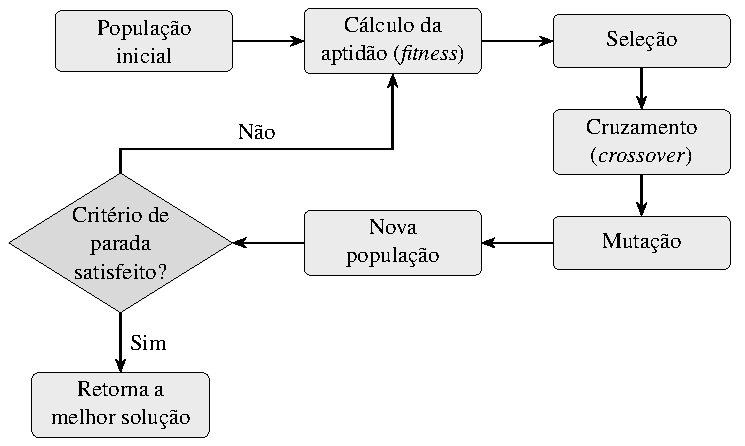
\includegraphics[width=0.7\textwidth]{figuras/diagramas/fluxograma_ag.pdf}
    \fonte{Elaboração própria, adaptado de \citeonline{linder2012}.}
\end{figure}

Na Programação Genética (PG), cada indivíduo é uma árvore sintática: os nós internos contêm funções ou operadores matemáticos, como adição, subtração e multiplicação, e as folhas contêm variáveis de entrada ou constantes. Diferentemente dos AG, que evoluem cromossomos numéricos de tamanho fixo, a PG evolui a própria estrutura do modelo, sem que o projetista precise definir previamente a sua forma \cite{pereda2020}. O cruzamento troca subárvores entre dois genitores, e a mutação substitui um ramo por uma nova subárvore aleatória, o que preserva a diversidade e reduz a convergência prematura \cite{willis1997}. Para limitar o crescimento excessivo das equações (\textit{bloat}), impõe-se uma profundidade máxima às árvores (\textit{maxHeight}); a seleção por torneio e o elitismo completam o processo \cite{koza2009}.

\section{Programação genética multigene e modelos NARX MIMO}\label{sec:mggp}

O MGGP surgiu para separar a busca heurística pela estrutura simbólica de um modelo não linear do ajuste numérico de seus coeficientes. Em vez de evoluir uma única árvore sintática, característica da PG, cada indivíduo no MGGP é formado por um conjunto de genes. Cada gene é representado por uma árvore matemática independente que combina variáveis de entrada e seus respectivos atrasos temporais por meio de operadores simbólicos.

Em cada geração, monta-se uma matriz de regressores que contém, em cada coluna, a avaliação da saída de um desses genes para as amostras do conjunto de treinamento. Em seguida, ajustam-se os coeficientes de ponderação ($\theta$) por meio do Método dos Mínimos Quadrados Ordinários (MQO), de modo que a combinação linear dos genes minimize o erro entre a saída do sistema e a predição. Esse procedimento atua na superfície de aptidão (\textit{fitness landscape}), pois o ajuste dos parâmetros lineares ($\theta$) é delegado a métodos de regressão, enquanto a evolução genética concentra-se em determinar quais genes devem compor o modelo \cite{pandey2015a, pereda2020}.

Os operadores genéticos no MGGP incluem o \textit{crossover} de alto nível, que permuta árvores completas (genes) entre os indivíduos progenitores, e o \textit{crossover} de baixo nível, que insere fragmentos de um progenitor dentro da árvore de outro. Adicionalmente, a mutação pode substituir um gene por uma nova árvore gerada aleatoriamente ou alterar uma subárvore interna, preservando parte da estrutura original \cite{koza2009, willis1997}.

Em problemas de identificação de sistemas dinâmicos, o MGGP é empregado na forma de modelos autorregressivos não lineares com entradas exógenas (NARX, do inglês \textit{Nonlinear AutoRegressive with eXogenous inputs}), em que a saída no instante $k$ depende de valores passados das entradas e das próprias saídas. Na arquitetura MIMO utilizada neste trabalho, cada indivíduo possui um conjunto próprio de genes para cada saída, e os valores atrasados de \emph{todas} as saídas estão disponíveis como terminais para \emph{todas} as árvores. Para uma saída $j$, o modelo assume a forma
\begin{equation}
    \hat y_j[k] = \theta_{j,0} + \sum_{i=1}^{n_T} \theta_{j,i}\, g_{j,i}\big(\mathbf{u}[k-d], \hat{\mathbf{y}}[k-d]\big),
    \label{eq:mggp_mimo}
\end{equation}
em que $n_T$ é o número de termos (genes) por saída, $g_{j,i}$ é o gene $i$ da saída $j$, e $d$ percorre o conjunto de atrasos permitidos. A \autoref{fig:individuo_mggp} ilustra um indivíduo com três saídas --- $\hat v_x$, $\hat v_y$ e $\hat\beta$ --- como os avaliados neste trabalho. Uma consequência importante dessa estrutura é que, quando $\beta$ é incluído como terceira saída, sua estimativa passa a poder ser usada pelas equações de $v_x$ e $v_y$, e vice-versa.

\begin{figure}[htbp]
    \centering
    \caption{Estrutura de um indivíduo MGGP NARX MIMO com três saídas. Cada saída é uma combinação linear de genes; as saídas atrasadas realimentam todas as árvores.}
    \label{fig:individuo_mggp}
    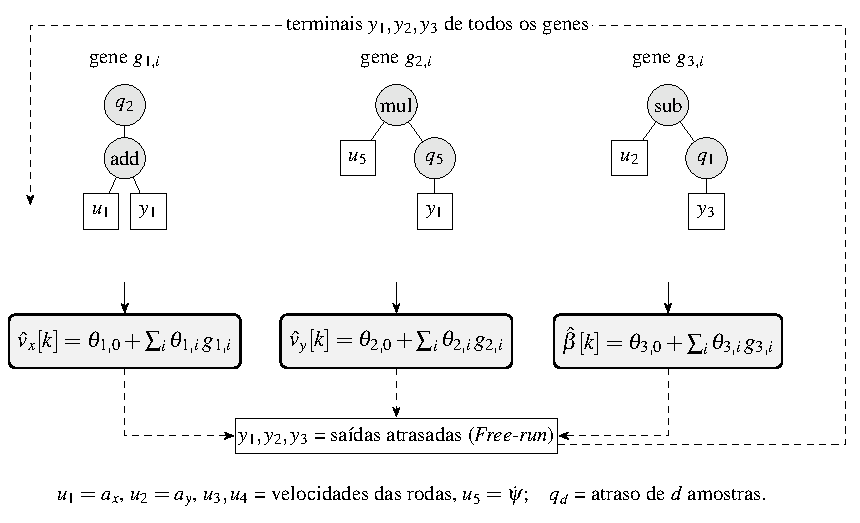
\includegraphics[width=\textwidth]{figuras/diagramas/individuo_mggp.pdf}
    \fonte{Elaboração própria.}
\end{figure}

Na biblioteca utilizada, a aptidão de um indivíduo MIMO é a média simples dos RMSE das saídas, sem normalização --- característica que se torna relevante quando as saídas têm escalas muito diferentes, como discutido na \autoref{sec:metodos}.

Aplicações em sistemas veiculares indicam que essa técnica pode ser utilizada para a construção de sensores virtuais, atendendo aos requisitos de análise na automação \cite{pandey2015a, mota2022, kaneko2022}.

\section{Regimes de simulação}\label{sec:regimes}

Em problemas de identificação de sistemas dinâmicos, adotam-se diferentes regimes de simulação e validação \cite{pandey2015a, kaneko2022}:

\begin{alineas}
    \item predição um passo à frente (\textit{one-step-ahead}): emprega os valores reais defasados do sistema para calcular a próxima predição, fornecendo resultados para análise inicial;
    \item simulação livre (\textit{free-run}): o modelo realimenta suas próprias predições passadas para gerar a sequência futura, evidenciando o comportamento do erro dinâmico ao longo do tempo. No caso MIMO, todas as saídas estimadas são realimentadas;
    \item tiros múltiplos (\textit{multi-shooting}): divide a série temporal em blocos de tamanho $K$, simulando livremente cada bloco e, ao final de cada intervalo, reinicia a predição com o valor real.
\end{alineas}

A simulação livre é o regime que corresponde à operação real de um sensor virtual, que não dispõe da medição da grandeza que estima; por isso, é o regime adotado em toda a avaliação deste trabalho \cite{castro2021}.
